\documentclass[svgnames]{beamer}
\usepackage{movie15}
\usepackage[french]{babel}
\usepackage[utf8]{inputenc}

%\usepackage[usenames,dvipsnames,svgnames,table]{xcolor}
% \mode<presentation>{\usetheme{Ilmenau}} % Ilmenau
% \mode<presentation>{\usetheme{Warsaw}} % Warsaw
\mode<presentation>{\usetheme{Frankfurt}} % Frankfurt
% \mode<presentation>{\usetheme{Darmstadt}} % Darmstadt

% toc before each section
% \AtBeginSection[]
% {
% \begin{frame}{Table of Contents}
% \tableofcontents[currentsection]
% \end{frame}
% }

% \AtBeginSection{\frame{\sectionpage}}
% \AtBeginSubsection{\frame{\subsectionpage}}
% \AtBeginSubsubsection{\frame{\subsubsectionpage}}

% add number of page
\beamertemplatenavigationsymbolsempty
\setbeamerfont{page number in head/foot}{}
\setbeamertemplate{footline}[frame number]

% progress bar
\useoutertheme{progressbar}
\progressbaroptions{titlepage=normal}
\progressbaroptions{headline=sections,frametitle=normal}


% add number of page
% \addtobeamertemplate{navigation symbols}{}{%
%     \usebeamerfont{footline}%
%     \usebeamercolor[fg]{footline}%
%     \hspace{1em}%
%     \insertframenumber/\inserttotalframenumber
% }

% remove symbols
\setbeamertemplate{navigation symbols}{}

% headers
\title{Kerberos}
\author{Laurentiu Capatina \& Quentin Lemaire}
\date{\today}

% content
\begin{document}
  
\maketitle % build title

% introduction
\section*{Introduction}

\begin{frame}
  \frametitle{Introduction}
  \begin{itemize}
    \item Cryptographie symétrique
    \item Serveur de distribution de clés
  \end{itemize}
\end{frame}

\begin{frame}
  \frametitle{Sommaire}
  \tableofcontents
\end{frame}

%% ------- %%

\section{Serveur de distribution de clés}

\begin{frame}
  \frametitle{Serveur de distribution de clés}
  \tableofcontents[currentsection, hideothersubsections]
\end{frame}


\subsection{Problème}
\begin{frame}
  \frametitle{Problème}
  
  \begin{center}
    Comment établir une clé de session entre 2 personnes ? % mutuellement authentifiées ?
  \end{center}
  
  \pause
  
  % DH ? Pas d'authentification
  \begin{alertblock}{Diffie Helman ?}
    Pas d'authentification
  \end{alertblock}
  
  \pause
  
  $\Rightarrow$ Utilisation d'un \textbf{tiers de confiance}
  
%   \begin{exampleblock}{Utilisation d'un tiers de confiance}
%     
%   \end{exampleblock}
\end{frame}


\subsection{Principe}
\begin{frame}
 \frametitle{Tiers de confiance}
% Un tiers de confiance possède toutes les clés et 
% sert à établir des communications entre les acteurs

  \begin{figure}[h!t]
    \begin{center}
      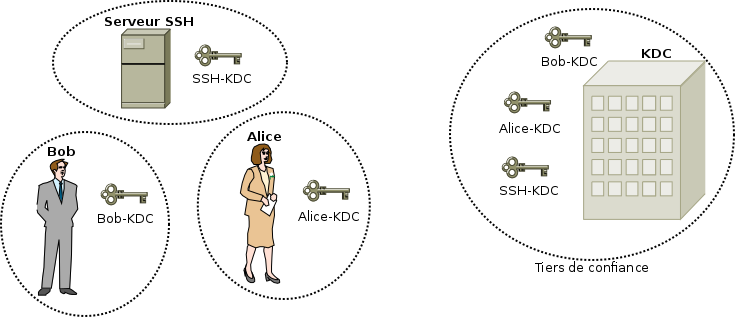
\includegraphics[width=\textwidth]{images/kdc.png} % KDC
      \caption{Serveur de Distribution de Clés (KDC en anglais)}
    \end{center}    
  \end{figure}

% - le KDC possède des clés partagées avec chaque utilisateur
% - le KDC s'occupe de mettre en relation les utilisateurs en fournissant
% des clés de session de manière sécurisée

% ==> OK mais comment on fait ?
\end{frame}

\subsection{Protocole Needham-Schroeder}
\begin{frame}
  \frametitle{Protocole Needham-Schroeder}

% explications : prévention du rejeu + mutal authentification

  \begin{figure}[h!t]
    \begin{center}
      \only<1>{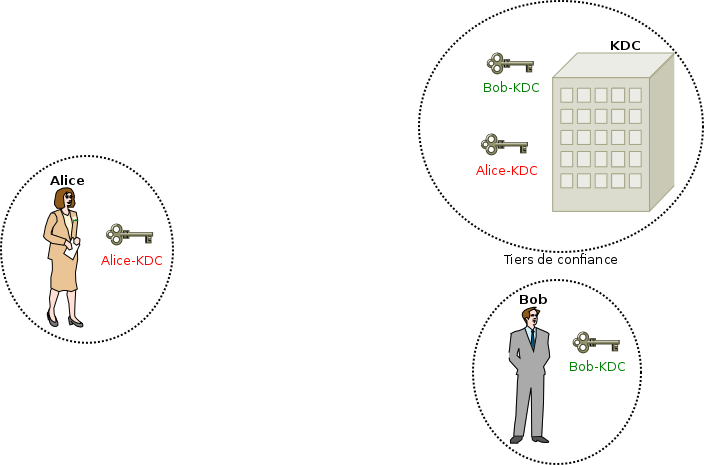
\includegraphics[width=0.9\textwidth]{images/needham_schroeder_1.png}} % actors
      \only<2>{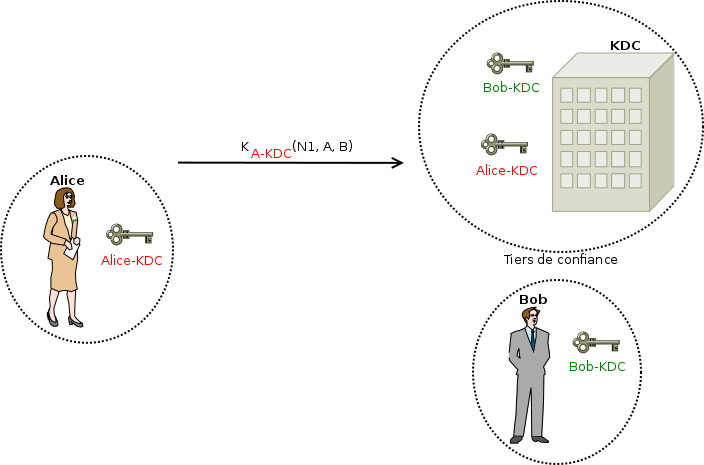
\includegraphics[width=0.9\textwidth]{images/needham_schroeder_2.png}} % 2
      \only<3>{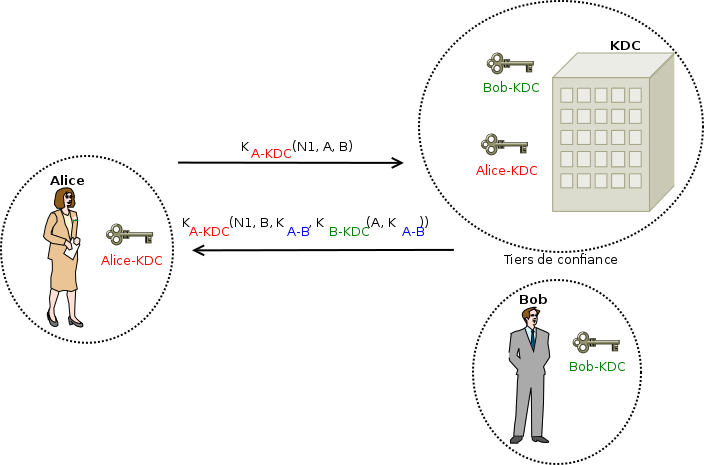
\includegraphics[width=0.9\textwidth]{images/needham_schroeder_3.png}} % 3
      \only<4>{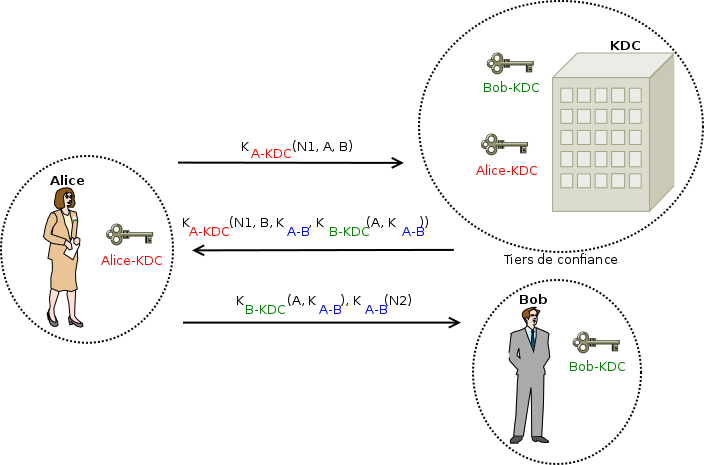
\includegraphics[width=0.9\textwidth]{images/needham_schroeder_4.png}} % 4
      \only<5>{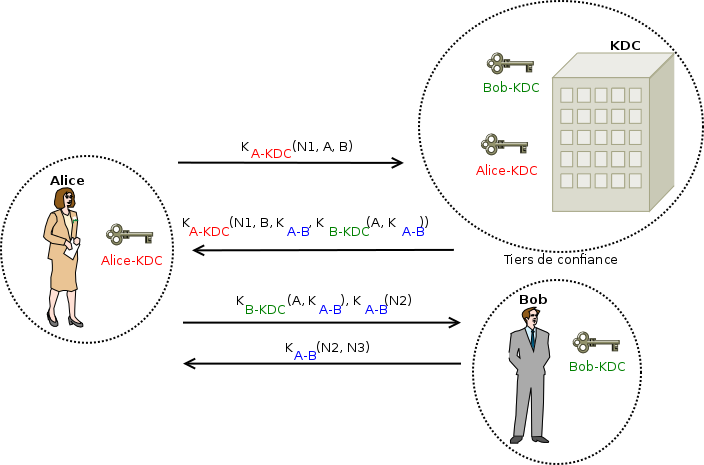
\includegraphics[width=0.9\textwidth]{images/needham_schroeder_5.png}} % 5
      \only<6>{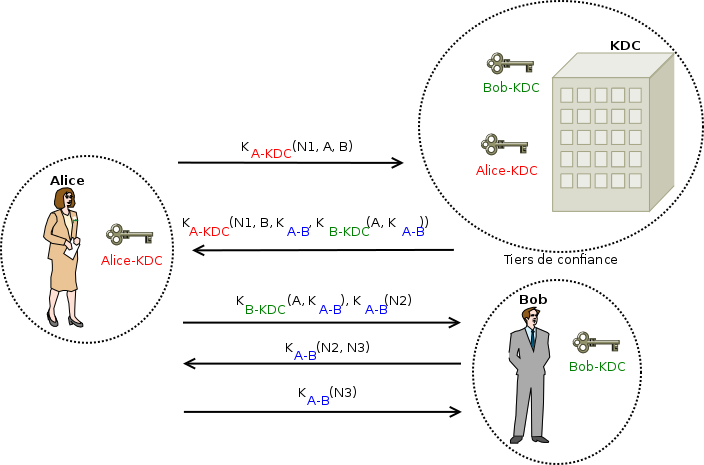
\includegraphics[width=0.9\textwidth]{images/needham_schroeder_6.png}} % 6
      \caption{Établissement d'une clé de session entre Alice et Bob.}
    \end{center}    
  \end{figure}

% TODO
% Problème de ce protocole :
% Invalidation de ticket => impossible de savoir si un 
% ticket est "neuf" si Alice se fait voler sa clé par 
% un attaquant
\end{frame}



% à partir de NS => Kerberos

\section{Kerberos}

\begin{frame}
  \frametitle{Kerberos}
  
  % Kerberos vient de "Cerbère" le chien qui garde les enfers
  % Projet initié par le MIT 
  % Protocole d'authentification basé sur le protocole NS
  % Utilisation de tickets
  % Évite de stocker des mots de passe en local et de les faire passer sur le réseau
  
  \tableofcontents[currentsection, hideothersubsections]
\end{frame}

\subsection{Protocole}

\begin{frame}
 \frametitle{Protocole : tickets}
 
  \begin{definition}
   Un ticket est une \textbf{preuve d'identité}.
   Chiffré avec la clé du service auprès duquel 
   l'utilisateur est authentifié. % => donc non forgeable
  \end{definition}
  
  \pause

  \vfill
  
  % Dans Kerberos =>
  Authentification en 2 étapes~:
  \begin{enumerate}
   \item Récupération d'un \textit{Ticket Granting Ticket} (TGT); % SSO
   \item Récupération de plusieurs \textit{Ticket Granting Service} (TGS) à l'aide du TGT. % Invisible pour l'utilisateur
  \end{enumerate}
  
\end{frame}

\begin{frame}
 \frametitle{Protocole : communications}
 % TODO diagramme 
%   2 serveurs dédiés~:
%   \begin{itemize}
%    \item \textit{Authentication Server} (AS) ;
%    \item \textit{Ticket Granting Server} (TGS).
%   \end{itemize}
\end{frame}


\begin{frame}
 \frametitle{Avantages \& Inconvénients}
 
% TODO avantages : SSO
% TODO inconvénients : 3rd party (tiers)
 
 % TODO
 \begin{exampleblock}{Avantages}
  \begin{itemize}
   \item Single-Sign-On (SSO) ;
   \item Les mots de passe ne passent pas par le réseau ;
  \end{itemize}
 \end{exampleblock}
 
 \pause
 
 % TODO
 \begin{alertblock}{Inconvénients}
  \begin{itemize}
   \item Tiers possédant l'ensemble des mots de passe ;
  \end{itemize}
 \end{alertblock}
\end{frame}

\subsection{Implémentations}

\begin{frame}
  \frametitle{Implémentations}
  
  % TODO séparer en 2 blocs
  \begin{itemize}
   \item MIT depuis XXXX : version 1.13.4 % TODO
   \item Heimdal depuis XXXX : version 1.5.2 % TODO
  \end{itemize}
  
  % TODO petite comparaison rapide et histoire des 2 implémentations principales
  
  % \pause
  % $\Rightarrow$ dans le cadre de la démonstration, utilisation de l'implémentation MIT de Kerberos version 5
\end{frame}


% TODO voir si on parle de toutes les attaques
\subsection{Attaques}

\begin{frame}
 \frametitle{Attaques}
 
 \begin{enumerate}
  \item Rejeu
  \item Vol de ticket
  \item Attaque offline par dictionnaire
 \end{enumerate}

\end{frame}

\begin{frame}
 \frametitle{Rejeu}
 
 % TODO schéma rapide : expliquer l'attaque
\end{frame}

\begin{frame}
 \frametitle{Vol de ticket}
 
 % Hôte non sécurisé
 
 %Pass the ticket
 \begin{block}{Pass-the-ticket}
  \begin{itemize}
   \item TGT ne contient pas l'identification physique de la machine émettrice
   \item Le transfer sur un autre poste permet toujours l'utilisation du TGT
  \end{itemize}
 \end{block}
 
 %Golden ticket
 \begin{block}{Golden ticket}
  \begin{itemize}
   \item Vulnérabilité découverte dans Active Directory
   \item Possibilité de générer des TGTs arbitraires après récuperation du hash KRBTGT
  \end{itemize}
 \end{block}
 % TODO révocation tickets Kerberos (regarder de la doc)
\end{frame}


\begin{frame}
 \frametitle{Attaque offline par dictionnaire}
   \begin{itemize}
   \item Envoi d'un message à l'AS
   \item Réponse est chiffré avec le mot de passe de l'utilisateur
   \item Utilisation d'un dictionnaire pour récupérer le mot de passe
  \end{itemize}
 % TODO explications:
 % 1- envoi d'un message à l'AS
 % 2- réponse par un message chiffré à l'aide du mot de passe de l'utilisateur usurpé
 % 3- attaque offline par dictionnaire pour récupérer le mot de passe 
 
 
 % => C'est cette attaque que nous allons vous montrer !
\end{frame}


\section{Démonstration}

\begin{frame}
  \frametitle{Démonstration}
  \tableofcontents[currentsection, hideothersubsections]
\end{frame}

\subsection{Récupération d'un mot de passe}
% TODO voir si on fait une vidéo
\begin{frame}
 \frametitle{Récupération d'un mot de passe}
 
 \begin{center}
  Démonstration !
  
  %  \begin{figure}[ht]
  %    \includemovie[poster,text={\small(Loading Video...)}]{6cm}{4cm}{media/video.avi}
  %  \end{figure}
 \end{center}
\end{frame}


\subsection{Comment s'en prémunir ?}

\begin{frame}
 \frametitle{Comment s'en prémunir ?}
 
 \begin{block}{Pré-authentification}
  \begin{itemize}
   \item Chiffrement du timestamp avec le mot de passe de l'utilisateur
   \item Vérification du timestamp contre un rejeu
   \item Syncronisation de l'heure des machines est obligatoire
  \end{itemize}
 \end{block}
 % TODO pre-auth
 % Implémentée depuis la version 5 MIT
\end{frame}

%% ------- %%

% Conclusion
\section*{Conclusion}
\begin{frame}
  \frametitle{Conclusion}
  
  \begin{exampleblock}{Atouts de Kerberos}
  \begin{itemize}
   \item Kerberos sert à faire de l'authentification
   \item Cela est réalisé à l'aide d'un tiers de confiance et sans le passage d'un mot de passe longue durée sur le réseau
     \end{itemize}
   \end{exampleblock}


  % TODO Kerberos sert à faire de l'authentification mais en aucun cas de l'autorisation.
  
  % TODO => souvent bindé avec un LDAP pour faire ça.
 \begin{alertblock}{Attention}
   \begin{itemize}
    \item Kerberos NE gère PAS l'autorisation!
    \item Cela doit être gerée au niveau applicatif
   \end{itemize}
  \end{alertblock}

\end{frame}


% Questions ?
\begin{frame}
  \frametitle{Merci}
  \begin{center}
    Merci pour votre attention. Question(s) ?
  \end{center}
\end{frame}

\end{document}